\FloatBarrier
\begin{figure*}[!t]
\centering
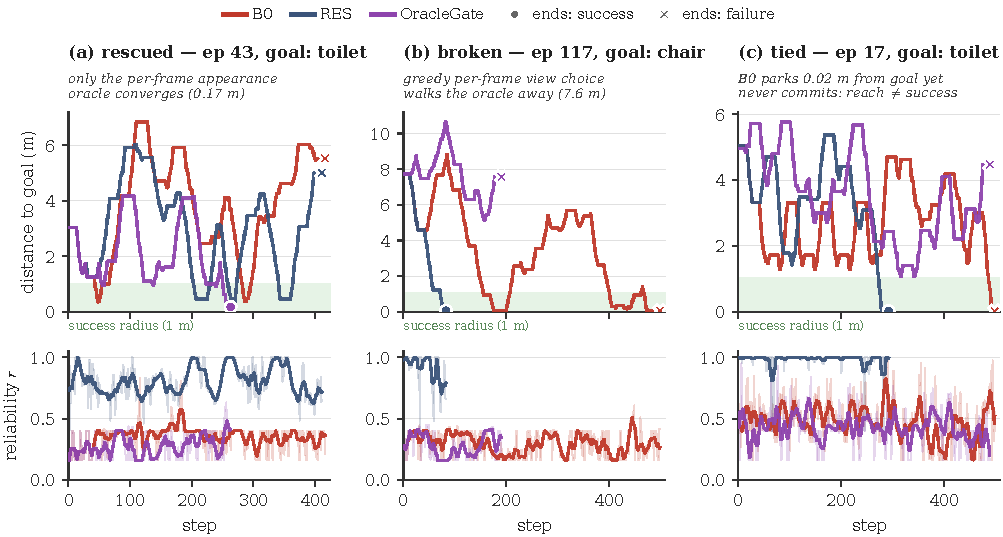
\includegraphics[width=0.68\textwidth]{figures/fig_case_studies.pdf}\\[2pt]
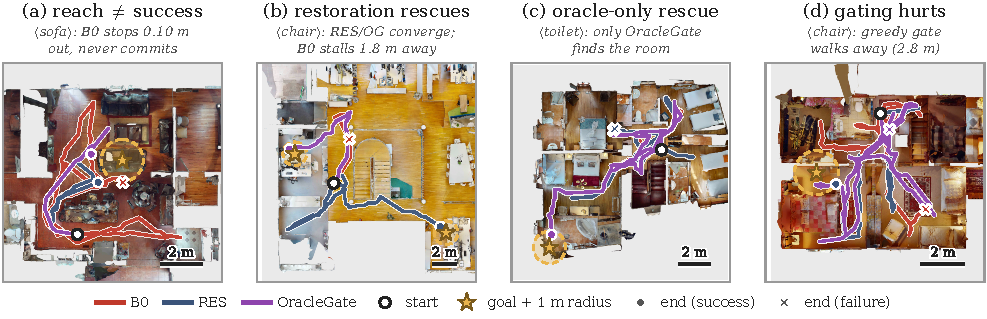
\includegraphics[width=0.68\textwidth]{figures/fig_trajectories.pdf}
\caption{\textbf{Episode-level views of the paired low-light cell.}
\emph{Top}: per-step distance to goal and reliability $r$ (B0, RES,
\textsc{OracleGate}, \emph{same} episode): a \emph{rescued}, a
\emph{broken}, and a \emph{tied} episode in which B0 touches $0.02$\,m
yet never commits---perception is restored, the decision is not.
\emph{Bottom}: top-down trajectories (stars: goal, $1$\,m radius).
Interventions reroute \emph{where} the agent goes far less than
\emph{whether} it commits.}
\label{fig:case-studies}
\label{fig:trajectories}
\end{figure*}

\begin{table*}[t]
\centering
\small
\setlength{\tabcolsep}{3.4pt}
\begin{tabular}{@{}lllcccccccc@{}}
\toprule
Family & Arm & What it does & SR$_{\text{B0}}$ & SR$_{\text{arm}}$ & $\Delta$SR & $\Delta$SPL & 95\% CI($\Delta$SR) & $p$ (McN.) & $N$ \\
\midrule
Appearance & RES & blanket restoration front-end & $0.370$ & $0.410$ & $+0.040$ & $+0.032$ & $[-0.013,+0.093]$ & $0.182$ & $300$ \\
Appearance UB & OracleGate$^{\ddagger}$ & per-frame best-of-two view & $0.370$ & $0.427$ & $\mathbf{+0.057}$ & $+0.025$ & $[+0.003,+0.110]$ & $\mathbf{0.043}$ & $300$ \\
Where-to-go & M1g & $r$-gated value-map reweight & $0.370$ & $0.410$ & $+0.040$ & $+0.012$ & $[-0.017,+0.097]$ & $0.201$ & $300$ \\
Commit timing & REVOKE & revoke stalled commitments & $0.380$ & $0.260$ & $\mathbf{-0.120}$ & $-0.020$ & $[-0.207,-0.040]$ & $\mathbf{0.006}$ & $150$ \\
Forced commit & CRV & close-range recall verifier & $0.380$ & $0.400$ & $+0.020$ & $+0.021$ & $[-0.053,+0.093]$ & $0.728$ & $150$ \\
Temporal & MUAP & hold-frames + re-observe & $0.380$ & $0.260$ & $\mathbf{-0.120}$ & $-0.039$ & $[-0.220,-0.020]$ & $\mathbf{0.022}$ & $150$ \\
Temporal & ROUTER & per-frame degradation router & $0.380$ & $0.393$ & $+0.013$ & $+0.031$ & $[-0.073,+0.100]$ & $0.875$ & $150$ \\
Multi-view & FUSE & multi-view identity fusion & $0.380$ & $0.367$ & $-0.013$ & $+0.032$ & $[-0.100,+0.073]$ & $0.878$ & $150$ \\
Multimodal probe & DXCV$^{\flat}$ & depth cross-modal veto & $0.380$ & $0.207$ & $\mathbf{-0.173}$ & $-0.057$ & $[-0.260,-0.087]$ & $\mathbf{{<}0.001}$ & $150$ \\
\bottomrule
\end{tabular}
\caption{\textbf{Intervention sweep across six causal families.} Paired protocol on low-light sev~$4$, seed~$0$, val split. The three top rows are scored at the $N{=}300$ main split; the six lower rows share a common $N{=}150$ subset with a single shared baseline, so all comparisons are on exactly the same episodes. Bold entries are significant at $p{<}0.05$ (McNemar exact). Every \emph{deployable} family either lands at a non-significant ${\sim}0$ or \emph{significantly hurts} success (REVOKE, MUAP, DXCV lower paired SR by $0.12$--$0.17$); the only arm clearing $p{<}0.05$ with a \emph{positive} $\Delta$SR is the non-deployable per-frame appearance upper bound, which caps at $+0.057$. Confidence intervals are $B{=}5000$ bootstrap over paired episode differences. $^{\ddagger}$non-deployable oracle. $^{\flat}$train-free depth-geometry cross-modal veto.}
\label{tab:sweep}
\end{table*}


\section{Experiments}
\label{sec:exp}

We now test the prediction of the diagnosis at scale. We first describe the
paired protocol, then report (i)~the degradation effect that defines the
benchmark, (ii)~two negative results that localize the bottleneck, (iii)~a
mechanism analysis that explains \emph{why} the candidates cap,
(iv)~evidence that the bottleneck resists a six-family intervention
sweep, and (v)~a
cross-corruption replication with a methodological warning about the
choice of sample size.

\subsection{Protocol}
We evaluate on HM3D ObjectNav with the InstructNav backbone
\citep{long2024instructnav}, using an open-source Qwen2-VL-7B-Instruct
\citep{wang2024qwen2vl} as the reasoning VLM (deterministic decoding on a
single RTX~5090; no external API), the GLEE open-vocabulary detector
\citep{wu2024glee} for segmentation, and InstructNav's value-map frontier
explorer for goal selection; the open-weight backbone makes every episode
re-runnable bit-identical from the released seeds. Conclusions are drawn
at the $N{=}300$ main-split scale; smaller runs serve only as pilots and
are never mixed with $N{=}300$ numbers. Each arm is run against the identical frozen baseline
(B0) on the same episodes, so comparisons are paired. We report success rate
(SR) and SPL, the paired per-episode difference $\Delta$SR, McNemar's exact test
on the discordant pairs, and a bootstrap $95\%$ CI over the paired differences
($B{=}5000$). Figure~\ref{fig:pipeline} (Appendix) illustrates the
instrument; the bottom strip of Figure~\ref{fig:method} previews the
four corruption channels. The primary degradation is low-light at severity~$4$, which
darkens the image while preserving geometry. Single-run point estimates
are avoided: the clean SR of the backbone alone ranges over
$0.27$--$0.53$ across seeds. Corruptions are injected into the RGB
stream only; depth, pose, and the episode specification are untouched,
so paired differences isolate the causal effect of the corrupted
visual input on navigation.

\subsection{The Degradation Effect (Benchmark)}
Structure-preserving degradation produces a large, real drop in
navigation success---the effect this benchmark studies. The M-study already
quantified it on the $n{=}90$ slice (paired drop $-0.211$, CI excluding
zero); at the $N{=}300$ main split the drop persists, from $0.44$ clean to
$0.37$ under low-light (McNemar $p{=}0.029$). Motion-blur at the same
severity gives $-0.056$ (CI $[-0.167,+0.056]$, not excluding zero), so
low-light is the primary condition and motion-blur a reported
non-significant case. The benchmark applies the same protocol at
multiple severities across all four corruption channels.

\subsection{Two Negative Results at $N{=}300$}
The diagnosis predicts two negative results---appearance (RES;
\textsc{OracleGate} is its upper bound) and where-to-go reweighting
(R-Weight)---and Table~\ref{tab:sweep} confirms both at $N{=}300$. Blanket restoration (RES) raises low-light SR from
$0.370$ to $0.410$, a paired $\Delta$SR of $+0.040$ that is not significant
($p{=}0.18$); the per-frame appearance oracle (\textsc{OracleGate})
reaches only $0.427$ ($+0.057$, $p{=}0.04$), indistinguishable from RES
($+0.017$);
reliability-gated where-to-go reweighting (R-Weight) also reaches
$+0.040$ ($p{=}0.20$). All three converge to the same
non-significant ${\sim}{+}0.04$, and no per-frame router over restored
versus degraded views can exceed the oracle.
Figure~\ref{fig:case-studies} grounds these aggregates in individual
episodes.

\subsection{Mechanism: Why the Candidates Cap}
The decomposition $\text{SR}=\text{reach}-\text{commit/stop loss}$ explains
the ceiling: across B0, RES, and R-Weight, reach (${\sim}0.62$) and commit/stop
loss (${\sim}0.23$) are nearly invariant, so no candidate changes whether
the agent reaches the goal or converts a reach into a stop. The per-episode
logs localize \emph{where} this invariance lives
(Figure~\ref{fig:decomp}, Appendix). First, the distance at which the agent
\emph{first commits} is unchanged by any intervention---the B0, RES, and
even OracleGate ECDFs coincide, with ${\sim}70\%$ of first commits firing
more than $3$\,m from the goal (Figure~\ref{fig:decomp}a). Second, RES
shifts the reliability distribution at those commit frames from a median
of $0.40$ to $1.00$, yet commit-to-success conversion moves only
$0.42\to0.43$ (Figure~\ref{fig:decomp}b). Third, the episodes that do flip
under RES were already at the $1$\,m margin under B0 (median $1.1$\,m):
the intervention perturbs threshold episodes rather than repairing far
failures (Figure~\ref{fig:decomp}c). Restoring perception without
repairing decision leaves the ${\sim}{+}0.04$ ceiling of
Table~\ref{tab:sweep}.

\subsection{The Bottleneck Resists a Six-Family Intervention Sweep}
\label{sec:sweep}
If the loss lived in a single module reachable by a layer-specific fix,
some arm of a broad sweep should move it. We sweep six causal
families (Table~\ref{tab:sweep}, visualized in Figure~\ref{fig:teaser}, right):
appearance (RES and its oracle upper bound), where-to-go
reweighting, commit-timing revocation, forced commitment,
temporal/multi-view aggregation, and a depth-based multimodal probe. The
six lower arms of Table~\ref{tab:sweep} are scored at a common $N{=}150$
on the same low-light severity~$4$ seed~$0$ episodes against the same
baseline, so comparisons are exactly paired. Every
\emph{deployable} family either lands at a non-significant ${\sim}0$
or \emph{significantly hurts} success: REVOKE, ReObserve and DepthVeto
lower paired SR by $0.12$--$0.17$ at $p{<}0.05$ (DepthVeto at
$p{<}0.001$); the only arm clearing $p{<}0.05$ with a \emph{positive}
$\Delta$SR is the non-deployable appearance oracle.
Crucially, accumulating evidence across frames, views, or
modalities can \emph{amplify} the wrong decision rather than repair it,
consistent with degradation suppressing the goal-distinguishing
evidence at the frame where the commitment fires.

\subsection{Probing the Multimodal Direction}
\label{sec:road2}
Is the bottleneck an RGB-specific problem that a degradation-invariant
sensing channel would dissolve? We test this with a train-free probe,
DepthVeto (a depth cross-modal verifier): when the VLM proposes
\texttt{Flag=True} at a low-reliability frame, a low-threshold GLEE pass
locates the target mask and the depth sensor must agree (thresholds in
Appendix~\ref{app:hp}), else the commit is vetoed and search resumes.
Habitat's depth is rendered from geometry, not light, so it is invariant
to low-light. Paired against the same $N{=}150$ baseline
(Table~\ref{tab:sweep}): $\Delta\text{SR}{=}{-}0.173$ (McNemar
$p{<}0.001$), the strongest negative effect in the sweep. Vetoing geometrically
implausible commits on a frozen agent removes true positives along with
the false ones: without a \emph{learned} joint RGB$+$depth representation
the verifier cannot tell them apart. A multimodal \emph{remedy}
therefore requires a detector \emph{trained} to fuse RGB with
depth---the training-side fix the Conclusion advocates.

\subsection{Cross-Corruption Replication}
\label{sec:cross-corruption}
A warning about scale first: on Gaussian noise an $N{=}40$ pilot yields
$\Delta\text{SR}{=}-0.125$ (RES apparently \emph{hurts}) while a matched
$N{=}150$ run collapses to $+0.000$ (Appendix~\ref{app:sample-size}), so
replication is run at matched scale. To rule out a low-light artefact, we
hold the InstructNav+Qwen2-VL-7B pipeline bit-identical and only swap the
corruption across low-light, motion-blur, fog, and Gaussian noise
(Table~\ref{tab:cross-corruption}, Appendix). No cell reaches significance at $\alpha{=}0.05$; the sign of
$\Delta\text{SR}$ flips between motion-blur ($-0.040$) and the other three
channels ($+0.000$--$+0.047$), reproducing the small-sample sign-flip
diagnosis above. The bottleneck is thus not a property of any one
corruption but of the \emph{commitment-on-degraded-input} interface
itself.

\paragraph{A first training-side probe.}
If the diagnosis is right, the lever should sit on the \emph{training}
side: a minimal probe---a $10^{6}$-parameter
residual adapter trained on scene-disjoint (clean,\,degraded) SwinL
feature pairs---moves degraded features $13.5\%$ closer to clean (L1)
and matches the best deployable arm of Table~\ref{tab:sweep}
($\Delta\text{SR}{=}{+}0.040$, $N{=}150$, $p{=}0.377$;
Appendix~\ref{app:road1}), though at pilot scale the effect is not
resolvable.
